\documentclass[11pt]{amsart}

\usepackage[utf8]{inputenc}
\usepackage{amsmath}
\usepackage{physics}
\usepackage{graphicx}
\usepackage{hyperref}
\usepackage[toc,page]{appendix}

% Custom colors
\usepackage{color}
\definecolor{deepblue}{rgb}{0,0,0.5}
\definecolor{deepred}{rgb}{0.6,0,0}
\definecolor{deepgreen}{rgb}{0,0.5,0}

\usepackage{listings}

% Python style for highlighting
\lstset{
language=Python,
basicstyle=\tiny,
otherkeywords={self, def},             % Add keywords here
keywordstyle=\tiny\color{deepblue},
emph={np,plt},          % Custom highlighting
emphstyle=\tiny\color{deepred},    % Custom highlighting style
stringstyle=\color{deepgreen},
frame=single,                         % Any extra options here
showstringspaces=false            % 
}

\renewcommand{\thesubsection}{\thesection.\alph{subsection}}

\title[Problem Sheet 4]{Hamiltonian Venture\\
	\hrulefill \small{ Problem Sheet 4: FYS3120 } \hrulefill}
	
\author[Winther-Larsen]{Sebastian G. Winther-Larsen}
\date{\today}

\begin{document}

\maketitle

\section{Constrained rod}

Figure \ref{fig:constrained_rod} shows a rod of lenth $b$ and evenly distributed mass $m$. One endpoint of the rod is constrained to move along a horizontal line, and the other endpoint is constrained to move along a vertical line. The two lines are in the same plane. There is no friction and the acceleration due to gravity is $g$.

\begin{figure}[ht]
\centering
	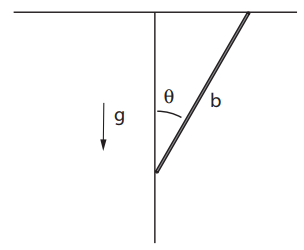
\includegraphics[width = 0.45\textwidth]{constrained_rod.png}
	\caption{Constrained rod}
	\label{fig:constrained_rod}
\end{figure}

\subsection{The Lagrangian and Lagrange's equation}
To fully describe the rod one needs one needs two translational coordinates and one rotational coordinate. The system has two constraints, so it is sufficient with one generalised coordinate, $\theta$, as the system only has one degree of freedom. The position of the left and right endpoint of the rod in terms of $\theta$ is
\begin{equation*}
(0, -b\cos \theta) \text{ and } (b\sin \theta, 0)
\end{equation*}
respectively. The position of the rods centre of mass must therefore be
\begin{equation}
\label{eq:com}
\vb{r} = (\frac{b}{2}\sin \theta, -\frac{b}{2}\cos \theta).
\end{equation}
It follows that 
\begin{equation*}
\dot{x} = \frac{b}{2}\dot{\theta}\cos \theta, \quad \dot{y} = \frac{b}{2}\dot{\theta}\sin \theta,
\end{equation*}
which gives
\begin{equation}
\label{eq:xandy}
\dot{x} + \dot{y} = \frac{b^2}{4}\dot{\theta}^2.
\end{equation}
The kinetic energy is the sum of translational and rotational energy\footnote{The moment of intertia for a rod rotating around its centre of mass is $I=\frac{mL^2}{12}$.}
\begin{equation}
\label{eq:travail1}
T 	= \frac{1}{2}m(\dot{x} + \dot{y}) + \frac{1}{2}I\dot{\theta}^2
	= \frac{1}{2}m\frac{b^2}{4}\dot{\theta}^2 + \frac{1}{2}\frac{mb^2}{12}
	= \frac{mb^2}{8}\dot{\theta}^2 + \frac{mb^2}{24}\dot{\theta}^2 
	= \frac{mb^2}{6}\dot{\theta}^2.
\end{equation}
The potential energy is
\begin{equation}
\label{eq:voltage1}
V 	= mgy = -\frac{1}{2}mg\cos \theta.
\end{equation}
The Lagrangian becomes
\begin{equation}
\label{eq:lagrangian1}
L = T - V = \frac{1}{6}mb^2\dot{\theta}^2 + \frac{1}{2}mgb \cos \theta 
\end{equation}

Lagrange's equation is given by
\begin{equation}
\label{eq:lagreqn}
\frac{d }{dt}\left(\frac{\partial L}{\partial \dot{\theta}} \right) - \frac{\partial L}{\partial \theta} = 0.
\end{equation}
Each part can be computed separately
\begin{align*}
\frac{\partial L}{\partial \theta} &= -\frac{1}{2} mgb \sin \theta \\
\frac{\partial L}{\partial \dot{\theta}} &= \frac{1}{3}mb^2\dot{\theta} \\
\frac{d }{dt}\left(\frac{\partial L}{\partial \dot{\theta}} \right) &= \frac{1}{3}mb^2 \ddot{\theta},
\end{align*}
and Lagrange's equation becomes
\begin{equation}
\frac{1}{3}mb^2\ddot{\theta} + \frac{1}{2}mgb \sin \theta = 0 \rightarrow 
\ddot{\theta} + \frac{3g}{2b}\sin \theta = 0
\end{equation}

\subsection{Equilibrium of the rod}
As usual, the system will tend towards a configuration where the potential, $V$, is as low as possible.  This point can be found by setting $\frac{\partial V}{\partial \theta} = 0$, but it is easy to see that it must be when $\theta = 0$.

When $\theta \to 0$, then $\sin \theta \to \theta$. Inserting this small-angle approximation into the Lagrange equation yields
\begin{equation}
\label{eq:lagapprox}
\ddot{\theta} + \frac{3g}{2b}\theta = 0,
\end{equation}
this equation corresponds to a harmonic oscillator with angular frequency $\omega = \sqrt{\frac{3g}{2b}}$. The period of an oscillation around the equilibrium orientation must then be
\begin{equation}
\label{eq:HOperiod}
T_0 = \frac{2\pi}{\omega} = 2\pi \sqrt{\frac{2b}{3g}}
\end{equation}

\subsection{Hamiltonian as constant of motion}
Since there $L$ has no explicit time dependence, there is a corresponding constant of motion. The Hamiltonian is related to the Lagrangian by the following equation
\begin{equation}
\label{eq:hamlang}
\frac{\partial H}{\partial t} = -\frac{\partial L}{\partial t} = 0.
\end{equation}
In this particular case the derivative of the Lagrangian with respect to time is equal to zero. It does not necessarily be so. The time derivative of the Hamiltonian must also be equal to zero, and is therefore a constant of motion. Now to find an expression for the Hamiltonian.
\begin{align}
H &= \sum_i \left( \frac{\partial L}{\partial \dot{q}_i} \dot{q}_i\right) - L \nonumber \\
 &= \frac{1}{3}mb^2\dot{\theta}^2 - \frac{1}{6}mb^2\dot{\theta}^2 - \frac{1}{2}mbg\cos\theta \nonumber \label{eq:hamiltonian} \\
 &= \frac{1}{6}mb^2\dot{\theta}^2 - \frac{1}{2}mbg\cos\theta \\
 &= T + V. \nonumber
\end{align}
One should take note that the Hamiltionian equals the total energy. The only force acting upon the system is gravity which is conservative. This implies that total energy is conserved, i.e. constant in time.

\subsection{Oscillation around equilibrium}
At the maximum angles $\theta_0$, the time derivative of the angle must be zero $\dot{\theta} = 0$. This reduces the Hamiltonian in this position to 
\begin{equation}
\label{eq:eqmHam}
H_0 = -\frac{1}{2}mbg \cos\theta_0.
\end{equation}
Because the energy i conserved (Hamiltonian is constant of motion) one can set expression \ref{eq:hamiltonian} equal to equation \ref{eq:eqmHam}.
\begin{align*}
H &= H_0 \\
\frac{1}{6}mb^2\dot{\theta}^2 - \frac{1}{2}mbg\cos\theta &= -\frac{1}{2}mbg\cos\theta_0 \\
\dot{\theta}^2 - \frac{3g}{2}\cos\theta &= - \frac{3g}{b}\cos\theta_0 \\
\frac{d\theta}{dt} = \dot{\theta} &= \pm \sqrt{\frac{3g}{b}}\sqrt{\cos\theta - \cos\theta_0} \\
\frac{dt}{d\theta} &= \pm \sqrt{\frac{b}{3g}} \frac{1}{\sqrt{\cos\theta - \cos\theta_0}}
\end{align*}
The last step will become apparent soon. From equation \ref{eq:HOperiod} one can set
\begin{equation}
\label{eq:H0period2}
\sqrt{\frac{b}{3g}} = T_0 \frac{1}{2\sqrt{2}\pi}
\end{equation}
which can be substituted into the expression above. The time it takes from the equilibrium position to the maximum angle is the sum of all infinitesimal angular displacements. Approximated by an integral this becomes
\begin{equation*}
T' = \int_0^{\theta_0}\frac{dt}{d\theta} d\theta = T_0 \frac{1}{2\sqrt{2}\pi}\int_0^{\theta_0}\frac{1}{\sqrt{\cos\theta - \cos\theta_0}}d\theta.
\end{equation*}
There are four such periods, $0 \to \theta_0$, $\theta_0 \to 0$, $0 \to -\theta_0$ and $-\theta_0 \to 0$. This means that the full period of the oscillatory motion is four times the integral above.
\begin{equation*}
T = 4T' = T_0 \frac{\sqrt{2}}{\pi} \int_0^{\theta_0}\frac{d\theta}{\sqrt{\cos\theta - \cos\theta_0}}.
\end{equation*}
The full space of ``swingable angles'' are included by setting $\theta_0 = \pi/2$
\begin{equation}
T = T_0\frac{\sqrt{2}}{\pi}\int_0^{\frac{\pi}{2}}\frac{d\theta}{\sqrt{\cos\theta}} = T_0\frac{\sqrt{2}}{\pi} \frac{\Gamma\left(\frac{1}{2} \right)\Gamma\left(\frac{1}{4} \right)}{2\Gamma\left(\frac{3}{4} \right)}
\end{equation}
the ratio $T/T_0$ becomes
\begin{equation}
\frac{T}{T_0} = \frac{1}{\sqrt{2}\pi}\frac{\Gamma\left(\frac{1}{2} \right)\Gamma\left(\frac{1}{4} \right)}{\Gamma\left(\frac{3}{4} \right)} \approx 1.18.
\end{equation}
I had to employ equation 103 on page 160 in K. Rottmann's collection of formulas and identities and a numerical solver to get here.

\section{Rotating pendulum}
A circular hoop is rotating with constant angular velocity $\omega$ around a symmetric axis with vertical orientation, as shown in figure \ref{fig:rotating_pendulum}. Inside the hoop a planar pendulum can perform free oscillations, while the plane of the pendulum rotates with the hoop. The mass of the pendulum bob is $m$, the length of the massless pendulum rod is $R$ and the gravitational acceleration is $g$. The angle $\theta$ of the pendulum relative to vertical axis is used as generalised coordinate.

\begin{figure}
\centering
	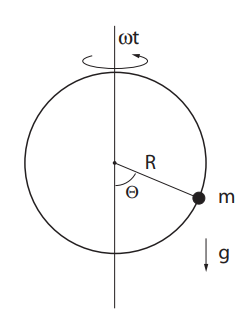
\includegraphics[width = 0.45\textwidth]{rotating_pendulum.png}
	\caption{Rotating pendulum}
	\label{fig:rotating_pendulum}
\end{figure}

\subsection{Lagrangian}
Spherical coordinates gives the position of the pendulum bob
\begin{align*}
x &= R\sin\theta\cos\omega t \\
y &= R\sin\theta\sin\omega t \\
z &= -R\cos\theta
\end{align*}
and the Cartesian coordinates' derivative in time is
\begin{align*}
\dot{x} &= R\dot{\theta}\cos\theta\cos\omega t - R\sin\theta\sin\omega t \\
\dot{y} &= R\dot{\theta}\cos\theta\sin\omega t + R\sin\theta\cos\omega t \\
\dot{z} &= R\dot{\theta}\sin\theta.
\end{align*}
The ``square sum'' of all this becomes
\begin{equation*}
\dot{x}^2 + \dot{y}^2 + \dot{z}^2 = R^2(\dot{\theta} + \omega^2\sin^2\theta)
\end{equation*}
and from this one can find the kinetic energy\footnote{Please see my answers for problem sheet 3 for a more thorough computation.}
\begin{equation}
\label{eq:KEpendulum}
T = \frac{1}{2}mR^2(\dot{\theta} + \omega^2\sin^2\theta),
\end{equation}
while potential energy is given by
\begin{equation}
\label{eq:PEpendulum}
T = mgz = -mgR\cos\theta.
\end{equation}
Equation \ref{eq:KEpendulum} and \ref{eq:PEpendulum} gives the Lagrangian
\begin{equation}
\label{eq:lagrangianpendulum}
L = T - V = \frac{1}{2}mR^2\dot{\theta}^2 + \frac{1}{2}m\omega^2R^2\sin\theta + mgR\cos\theta
 = \frac{1}{2}mR^2\dot{\theta}^2 - W(\theta),
\end{equation}
where 
\begin{equation*}
W(\theta) = -\left(\frac{1}{2}m\omega^2 R^2\sin^2\theta + \frac{1}{2}mgR\cos\theta\right)
\end{equation*}
is the effective potential. The term which is not there because of gravity is the fictitious centrifugal force. 


\subsection{Lagrange's equation}
.. given by the expression in \ref{eq:lagreqn}.
\begin{align*}
\frac{\partial L}{\partial \theta} &= m\omega^2R^2\cos\theta\sin\theta - mgR\sin\theta \\
\frac{\partial L}{\partial \dot{\theta}} &= mR^2\dot{\theta} \\
\frac{d}{dt}\left(\frac{\partial L}{\partial \dot{\theta}} \right)
&= mR^2\ddot{\theta}.
\end{align*}
All this gives Lagrange's equation as
\begin{align*}
mR^2\ddot{\theta} - \frac{1}{2}m\omega^2R^2\cos\theta\sin\theta + mgR\sin\theta &= 0 \\
\ddot{\theta} - \omega^2\cos\theta\sin\theta + \frac{g}{R}\sin\theta &= 0.
\end{align*}
If $\theta \to 0$ then $\cos\theta \to 1$, $\sin\theta \to \theta$ so that the Lagrange equation reduces to
\begin{equation}
\label{eq:oscillatorpen}
\ddot{\theta} + \theta\left(\frac{g}{R}-\omega^2 \right) = 0
\end{equation}
which corresponds to a harmonic oscillator with frequency
\begin{equation*}
\Omega = \sqrt{\frac{g}{R}-\omega^2}
\end{equation*}

\subsection{Stable equilibria and critical angular velocity}
The solution for equation \ref{eq:oscillatorpen} is stable if
\begin{equation*}
\frac{g}{R}-\omega^2 > 0
\end{equation*}
and unstable if
\begin{equation*}
\frac{g}{R}-\omega^2 < 0.
\end{equation*}
The critical angular velocity, $\omega_{cr}$ is given by
\begin{equation}
\frac{g}{R}-\omega_{cr}^2 = 0 \rightarrow \omega_{cr} = \sqrt{\frac{g}{R}}.
\end{equation}
The equilibrium points are extremal points of the potential $W(\theta)$, satisfying
\begin{equation*}
\frac{\partial W}{\partial \theta} = 0.
\end{equation*}
Differentiating gives
\begin{equation}
\frac{\partial W}{\partial \theta} = \frac{g}{R}\sin\theta - \omega^2\sin\theta\cos\theta
\end{equation}
which is zero either if $\sin\theta = 0$, which gives the points $\theta = 0,\pi$, or if $\omega^2\cos\theta = \frac{g}{R}$, which gives 
\begin{equation}
\label{eq:thetapm}
\theta_\pm = \cos^{-1}\frac{g}{\omega^2R}. 
\end{equation}
These last points are only valid for
\begin{equation*}
\frac{g}{\omega^2R} < 1 \rightarrow \frac{g}{R} < \omega^2 \rightarrow \omega_{cr} < \omega. 
\end{equation*}
These last two points are the interesting ones.

\subsection{Stability of equilibrium points}
The stability of $\theta_\pm$ in \ref{eq:thetapm} can be determined by the ``second-derivative test''. One would want them to be minima, satisfying
\begin{equation*}
\frac{\partial^2 W}{\partial \theta^2} > 0.
\end{equation*}
Computing,
\begin{align*}
\frac{\partial^2 W}{\partial \theta^2} 
&= \frac{\partial}{\partial \theta} \left(\frac{g}{R}\sin\theta - \omega^2\cos\theta\sin\theta \right)\\
&= \frac{g}{R}\cos\theta - \omega(\cos^2\theta-\sin^2\theta),
\end{align*}
inserting $\theta_\pm$,
\begin{align*}
\frac{\partial^2 W}{\partial \theta^2} 
&= \frac{g}{R}\frac{g}{\omega^2R}-\omega^2\left(\frac{g^2}{\omega^4R^2} - 1 + \frac{g^2}{\omega^4R^2} \right) \\
&= \frac{g^2}{R^2\omega^2} - 2\frac{g^2}{R^2\omega^2} + \omega^2 \\
&=\omega^2 - \frac{g^2}{R^2\omega^2} = \omega^2 - \frac{\omega_{cr}^4}{\omega^2} > 0\\
&\rightarrow \omega > \omega_{cr}
\end{align*}
This means that the points in \ref{eq:thetapm} are minima and therefore stable.

\begin{figure}
\centering
	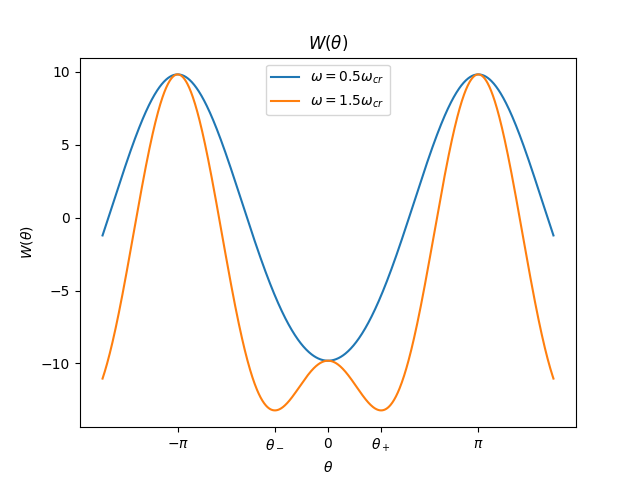
\includegraphics[width=0.75\textwidth]{critical_omega.png}
	\caption{The effective potential for different angular velocities}
	\label{fig:angvel}
\end{figure}

Figure \ref{fig:angvel} shows the effective potential $W{\theta}$ for different angualar velocities $\omega = 0.5\omega_{cr}$ and $\omega = 1.5\omega_{cr}$. There are obvious local maxima at $-\pi$ and $\pi$, and a minimum at $0$. Only for $\omega > \omega_{cr}$ are there minima between $0$ and $\pi$. 

\subsection{The Hamiltonian}
The Hamiltonian is defined by
\begin{align*}
H &= p_\theta - L = \frac{\partial L}{\partial \dot{\theta}}\dot{\theta} - L\\
  &= mR^2\dot{\theta}^2 - L = \frac{1}{2}mR^2\dot{\theta}^2 + W(\theta) \\
  &= T + W(\theta),
\end{align*}
which is the total energy and should be conserved in the presence of nothing else than conservative forces. Gravity is a conservative force, but the fictitious centrifugal force warrants further investigation. The centrifugal force does work which is might lead one to believe that it \emph{is} non-conservative, but it only depends on position, not velocity, and therefore is not. Also since there is no explicit time dependence
\begin{equation}
\frac{\partial H}{\partial t} = -\frac{\partial L}{\partial t} = 0,
\end{equation}
which leads one to conclude that the Hamiltonian is a constant of motion.

\subsection{Phase space}
\begin{figure}
\centering
	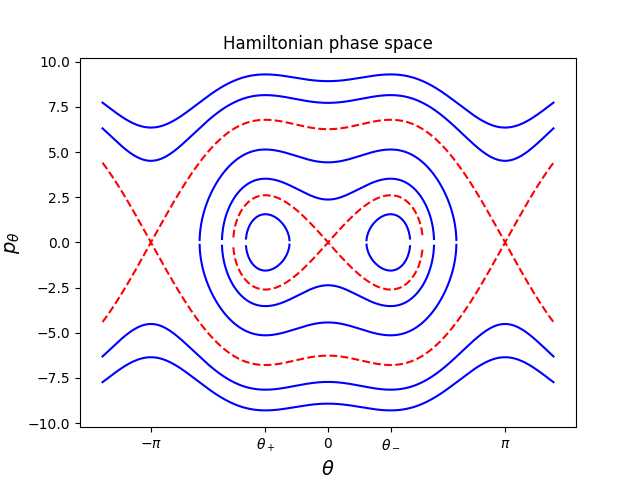
\includegraphics[width = 0.75\textwidth]{phase_space.png}
	\caption{Hamiltonian phase space displaying three kinds of motions for the system separated by dashed, red lines. The angular velocity is $\omega = 1.5\omega_{cr}$, making stable equilibria possible for angles larger than zero.}
	\label{fig:phasespace}
\end{figure}

Figure \ref{fig:phasespace} shows the equipotential lines of the Hamiltonian as a function of position and conjugate momentum $H(\theta, p_\theta)$. A function for these lines can be found by rewriting the equation for the Hamiltonian
\begin{align*}
H &= \frac{1}{2}mR^2\dot{\theta}^2 - \frac{1}{2}mR^2\omega^2\sin^2\theta - mgR\cos\theta \\
  &= \frac{1}{2}\frac{1}{mR^2}p_\theta^2 - \frac{1}{2}mR^2\omega^2\sin^2\theta - mgR\cos\theta\\
\rightarrow P_\theta^2 &= 2mR^2(H - W(\theta)) \\
P_\theta^2  &= \pm R \sqrt{2mH + (mR\omega\sin\theta)^2 + 2gm^2R\cos\theta)}.
\end{align*}

The plot in figure \ref{fig:phasespace} shows three kinds of motions,
\begin{itemize}
\item Motion around one equilibrium position, indicated by the small, blue circular graphs in the middle of the plot,
\item Motion around two equilibria, indicated in the figure as the blue loops between the two red, dashed loops, and
\item Unbounded, unoscillatory motion which are the wavy lines on the top and bottom of plot.
\end{itemize}
The motion in the phase space is given by the gradient and is clockwise in the figure.


\begin{appendices}
\section{Critical angular velocity script}
\lstinputlisting[language=Python]{critical_omega.py}

\section{Phase space script}
\lstinputlisting[language=Python]{phase_space.py}


\end{appendices}



\end{document}

